\documentclass{../zirkelblatt1415}

\pagestyle{empty}

\begin{document}

\begin{aufgabe}{Gerade Zahlen}
\begin{enumerate}
 \item Rechne die Zahl $n^2 + n$ f\"ur $n = 1,2,3,\ldots$ aus. Was stellst du fest?
 \item Beweise deine Vermutung mit Induktion.
 \item Es gibt auch noch andere, anschauliche Beweise f\"ur diese Aussage. F\"allt dir dazu etwas ein?
\end{enumerate}\fixlistspacing
\end{aufgabe}

\begin{aufgabe}{Eine falsche Induktion}
Ich werde euch nun mit Induktion beweisen, dass alle Katzen die gleiche Farbe haben.

Beginnen wir mit dem Induktionsanfang, den Fall einer einzigen Katze.
Diese hat nat\"urlich die gleiche Farbe wie sie selbst. Das ist sehr einfach, da haben wir gar nichts zu tun.

Die Induktionsvoraussetzung sei nun, dass eine Menge von $n$ Katzen stets die gleiche Farbe hat.
Nun geht es an die Arbeit: Nehmen wir uns jetzt eine Menge von $n+1$ Katzen vor.
Wir k\"onnen die Katzen aufteilen. Eine Katze trennen wir erstmal vom Rest, dann bleibt eine Menge von $n$ Karten \"ubrig.
Prima, diese haben also alle dieselbe Farbe, nach Induktionsvoraussetzung.
Aber \"uber die einzelne Katze wissen wir noch nichts. Deshalb machen wir das so:
Wir vereinen wieder alle Katzen und trennen diesmal eine andere als zuvor vom Rest.
Die verbleibenden $n$ Katzen haben auch alle dieselbe Farbe -- und da diesmal die vorher einzelne Katze dabei ist, 
haben jetzt also alle $n+1$ Katzen die gleiche Farbe.
Prima!

Und jetzt kommt ihr ins Spiel: Da offensichtlich nicht alle Katzen auf der Welt die gleiche Farbe haben -- 
was ist an diesem Beweis falsch?
\end{aufgabe}

\begin{aufgabe}{Ungerade Zahlen}
Wir wollen jetzt nur ungerade Zahlen betrachten.
\begin{enumerate}
\item Addiere doch mal die ersten $1, 2, 3, \ldots$ ungeraden Zahlen. Was kommt dabei heraus?
\item Was kommt heraus, wenn man die ersten $n$ ungeraden Zahlen addiert? 
\item Beweise diese Vermutung mit Induktion. Dabei ist es hilfreich zu wissen, dass die $n$-te ungerade Zahl $2n-1$ ist.
      Warum ist das so?
\item Auch hier gibt es eine anschauliche Beweismethode ohne Induktion. Vielleicht f\"allt dir ja etwas ein.      
\end{enumerate}\fixlistspacing
\end{aufgabe}

\newpage

\begin{aufgabe}{Pascalsches Dreieck}
Addiere mal die einzelnen Zeilen im Pascalschen Dreieck.
\begin{center}
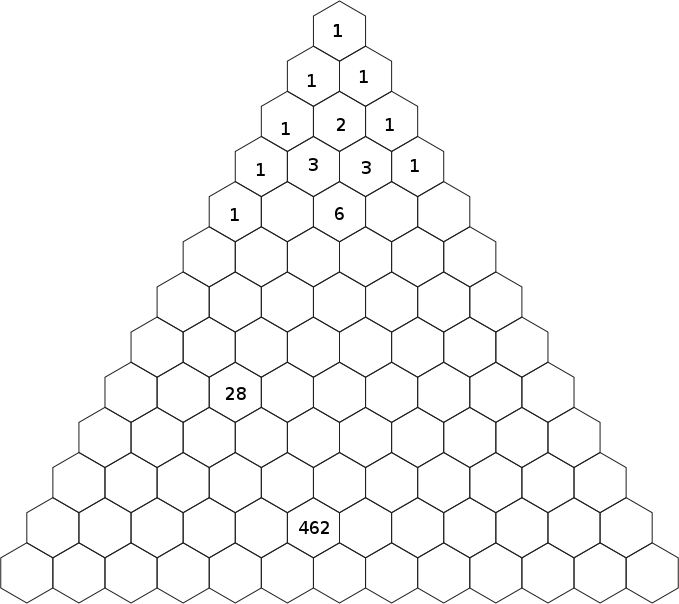
\includegraphics[scale=0.8]{pascal-triangle-tipps}
\end{center}
\begin{enumerate}
\item Was f\"allt dir auf? Und was hat das mit $2^n$ zu tun?
\item Beweise deine Vermutung mit Induktion!
\end{enumerate}\fixlistspacing
\end{aufgabe}

\begin{aufgabe}{Rekursive Folgen}
Wir betrachten die folgende Zahlenfolge
\begin{align*}
a_1 = 1, \quad a_2 = 4, \quad a_3 = 13, \quad a_4 = 40, \quad \ldots,
\end{align*}
die n\"achste Zahl ist also immer Eins mehr als das Dreifache der vorherigen
Zahl. Als Formel:
\begin{align*}
 a_{n+1} = 3 a_n + 1.
\end{align*}
Beweise mit Induktion, dass $a_n = \frac{3^n - 1}{2}$.
\end{aufgabe}

 \begin{aufgabe}{Triominos}
Beweise mit Induktion: Ein $(2^n \times 2^n)$-Schachbrett kann so mit Triominos belegt werden, dass die obere rechte Ecke frei bleibt 
und sonst alle Felder mit genau einem Triomino belegt sind. (Wie in der Skizze f\"ur $n=3$.)

\begin{center}
 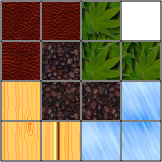
\includegraphics[scale=1]{triominos.png}
\end{center}

\noindent Tipp: Aus wie vielen $(2^n \times 2^n)$-Teilbrettern besteht ein $(2^{n+1} \times 2^{n+1})$-Brett?
 \end{aufgabe}

\begin{aufgabe}{Multiplikation}
Beweise mit Induktion: 
\begin{align*}
\left(1 - \frac{1}{4}\right) \cdot \left(1 - \frac{1}{9}\right) \cdot \left(1 -
\frac{1}{16}\right) \cdot \ldots \cdot \left(1 - \frac{1}{n^2}\right) = \frac{n+1}{2n}.
\end{align*}
\vspace{-1em}
\end{aufgabe}

\begin{aufgabe}{Eine absurde Gleichung}
Beweise mit Induktion:
\begin{align*}
(1 + 2 + 3 + \cdots + n)^2 = 1^3 + 2^3 + 3^3 + \cdots + n^3.
\end{align*}
\vspace{-2em}
\end{aufgabe}

\enlargethispage{2.5em}

\begin{aufgabe}{Fibonacci-Zahlen}
In dieser Aufgabe besch\"aftigen wir uns mit den \emph{Fibonacci-Zahlen}.
Das sind die Zahlen
\[ f_1 = 1, \quad f_2 = 1, \quad f_3 = 2, \quad f_4 = 3, \quad f_5 = 5,
\quad f_6 = 8, \quad f_7 = 13, \quad f_8 = 21, \quad \ldots, \]
die n\"achste Zahl ist also immer die Summe der beiden vorhergehenden
Zahlen.
\begin{enumerate}
\item Beweise mit Induktion:
$f_1 + f_2 + f_3 + \cdots + f_n = f_{n+2} - 1$.
\item Versuch mal den Induktionsschritt bei folgender (unsinniger) Behauptung! \\
$f_1 + f_2 + f_3 + \cdots + f_n = f_{n+2} - 17$.
\item Beweise mit Induktion:
$f_1^2 + f_2^2 + f_3^2 + \cdots + f_n^2 = f_n \cdot f_{n+1}$.
\end{enumerate}\fixlistspacing
\end{aufgabe}

\end{document}

\begin{aufgabe}{Eine mathematische Party}
Auf einer mathematischen Party möchten sich alle Gäste gegenseitig mit
Handschlag begrüßen. Jeder Gast möchte also jedem anderem Gast genau
einmal die Hand geben. Beweise mit Induktion: Bei~$n$ Gästen gibt es
insgesamt~$\frac{1}{2} \cdot n \cdot (n-1)$ viele Handschläge.
\end{aufgabe}
